\documentclass[final]{beamer}\usepackage[]{graphicx}\usepackage[]{color}
%% maxwidth is the original width if it is less than linewidth
%% otherwise use linewidth (to make sure the graphics do not exceed the margin)
\makeatletter
\def\maxwidth{ %
  \ifdim\Gin@nat@width>\linewidth
    \linewidth
  \else
    \Gin@nat@width
  \fi
}
\makeatother

\definecolor{fgcolor}{rgb}{0.345, 0.345, 0.345}
\newcommand{\hlnum}[1]{\textcolor[rgb]{0.686,0.059,0.569}{#1}}%
\newcommand{\hlstr}[1]{\textcolor[rgb]{0.192,0.494,0.8}{#1}}%
\newcommand{\hlcom}[1]{\textcolor[rgb]{0.678,0.584,0.686}{\textit{#1}}}%
\newcommand{\hlopt}[1]{\textcolor[rgb]{0,0,0}{#1}}%
\newcommand{\hlstd}[1]{\textcolor[rgb]{0.345,0.345,0.345}{#1}}%
\newcommand{\hlkwa}[1]{\textcolor[rgb]{0.161,0.373,0.58}{\textbf{#1}}}%
\newcommand{\hlkwb}[1]{\textcolor[rgb]{0.69,0.353,0.396}{#1}}%
\newcommand{\hlkwc}[1]{\textcolor[rgb]{0.333,0.667,0.333}{#1}}%
\newcommand{\hlkwd}[1]{\textcolor[rgb]{0.737,0.353,0.396}{\textbf{#1}}}%

\usepackage{framed}
\makeatletter
\newenvironment{kframe}{%
 \def\at@end@of@kframe{}%
 \ifinner\ifhmode%
  \def\at@end@of@kframe{\end{minipage}}%
  \begin{minipage}{\columnwidth}%
 \fi\fi%
 \def\FrameCommand##1{\hskip\@totalleftmargin \hskip-\fboxsep
 \colorbox{shadecolor}{##1}\hskip-\fboxsep
     % There is no \\@totalrightmargin, so:
     \hskip-\linewidth \hskip-\@totalleftmargin \hskip\columnwidth}%
 \MakeFramed {\advance\hsize-\width
   \@totalleftmargin\z@ \linewidth\hsize
   \@setminipage}}%
 {\par\unskip\endMakeFramed%
 \at@end@of@kframe}
\makeatother

\definecolor{shadecolor}{rgb}{.97, .97, .97}
\definecolor{messagecolor}{rgb}{0, 0, 0}
\definecolor{warningcolor}{rgb}{1, 0, 1}
\definecolor{errorcolor}{rgb}{1, 0, 0}
\newenvironment{knitrout}{}{} % an empty environment to be redefined in TeX

\usepackage{alltt}
\usepackage{grffile}
\mode<presentation>{\usetheme{CambridgeUSPOL}}

\usepackage[utf8]{inputenc}
\usepackage{amsfonts}
\usepackage{amsmath}
\usepackage{natbib}
\usepackage{graphicx}
\usepackage{array,booktabs,tabularx}
\usepackage{colortbl, xcolor}
\newcolumntype{Z}{>{\centering\arraybackslash}X}

% rysunki
\usepackage{tikz}
\usepackage{ifthen}
\usepackage{xxcolor}
\usetikzlibrary{arrows}
\usetikzlibrary[topaths]
\usetikzlibrary{decorations.pathreplacing}
%\usepackage{times}\usefonttheme{professionalfonts}  % times is obsolete
\usefonttheme[onlymath]{serif}
\boldmath
\usepackage[orientation=portrait,size=a0,scale=1.4,debug]{beamerposter}                       % e.g. for DIN-A0 poster
%\usepackage[orientation=portrait,size=a1,scale=1.4,grid,debug]{beamerposter}                  % e.g. for DIN-A1 poster, with optional grid and debug output
%\usepackage[size=custom,width=200,height=120,scale=2,debug]{beamerposter}                     % e.g. for custom size poster
%\usepackage[orientation=portrait,size=a0,scale=1.0,printer=rwth-glossy-uv.df]{beamerposter}   % e.g. for DIN-A0 poster with rwth-glossy-uv printer check
% ...
%

\usecolortheme{seagull}
\useinnertheme{rectangles}
\setbeamercolor{item projected}{bg=darkred}
% \setbeamertemplate{enumerate items}[default]
\setbeamertemplate{caption}{\insertcaption} 
\setbeamertemplate{navigation symbols}{}
\setbeamercovered{transparent}
\setbeamercolor{block title}{fg=darkred}
\setbeamercolor{local structure}{fg=darkred}

\setbeamercolor*{enumerate item}{fg=darkred}
\setbeamercolor*{enumerate subitem}{fg=darkred}
\setbeamercolor*{enumerate subsubitem}{fg=darkred}

\setbeamercolor*{itemize item}{fg=darkred}
\setbeamercolor*{itemize subitem}{fg=darkred}
\setbeamercolor*{itemize subsubitem}{fg=darkred}

\newlength{\columnheight}
\setlength{\columnheight}{96cm}
\renewcommand{\thetable}{}
\def\andname{,}
\authornote{}

\renewcommand{\APACrefatitle}[2]{}
\renewcommand{\bibliographytypesize}{\footnotesize} 
\renewcommand{\APACrefYearMonthDay}[3]{%
  {\BBOP}{#1}
  {\BBCP}
}
\IfFileExists{upquote.sty}{\usepackage{upquote}}{}
\begin{document}







\date{}
\author{Micha\l{} Burdukiewicz\inst{1}, Piotr Sobczyk\inst{2}, Pawe\l{} Mackiewicz\inst{1} and Ma\l{}gorzata Kotulska\inst{3}
}


\institute{\small{\textsuperscript{1}University of Wroc\l{}aw, Department of Genomics, Poland 

\vspace{0.3cm}

\textsuperscript{2}Wroc\l{}aw University of Technology, Department of Mathematics, Poland

\vspace{0.3cm}

\textsuperscript{3}Wroc\l{}aw University of Technology, Department of Biomedical Engineering, Poland}
}
}
\title{\huge N-gram analysis of amyloid data}

\begin{frame}
\begin{columns}
\begin{column}{.50\textwidth}
\begin{beamercolorbox}[center,wd=\textwidth]{postercolumn}
\begin{minipage}[T]{.95\textwidth}
\parbox[t][\columnheight]{\textwidth}
{
\begin{block}{Aim}
Investigate and predict sequences responsible for amyloidogenicity, the cause of various clinical disorders (e.g. Alzheimer's or Creutzfeldt-Jakob's diseases).
\end{block}
\vfill

\begin{block}{Introduction}
All amyloidogenic sequences (amyloids), despite their variability in size and amino acid composition, form mostly cytotoxic aggregates~\citep{breydo_structural_2015}. The hallmark trait of amyloids is the presence of hot-spots, short sequences of amino acids that play key role in the aggregation process~\citep{fandrich_oligomeric_2012}.
\end{block}
\vfill


\begin{block}{AmyLoad database}


The sequences used in the study (1044 non-amyloids and 421 amyloids) were extracted from AmyLoad database~\citep{wozniak_amyload:_2015}.

\begin{knitrout}
\definecolor{shadecolor}{rgb}{0.969, 0.969, 0.969}\color{fgcolor}
\includegraphics[width=\maxwidth]{figure/AmyLoadPlot-1} 

\end{knitrout}


\end{block}
\vfill



\begin{block}{Clustering of amino acids}

\begin{enumerate}[1.]
\item Nine scales representing properties important in the amylogenicity: hydrophobicity, size polarity and solvent accessibility from AAIndex database~\citep{kawashima_aaindex:_2008} were chosen. Additionally, two frequencies of forming contact sites~\citep{wozniak_characteristics_2014} were added. All scales were normalized.
\item All combinations of characteristics (each time selecting only one scale per the property) were clustered using Euclidean distance and Ward's method.
\item Each clustering was divided into 3 to 6 groups creating 144 encodings of amino acids.
\item Redundant 51 encodings (identical to other encodings) were removed.
\end{enumerate}

\end{block}
\vfill

\begin{block}{Evaluation}

\begin{figure}
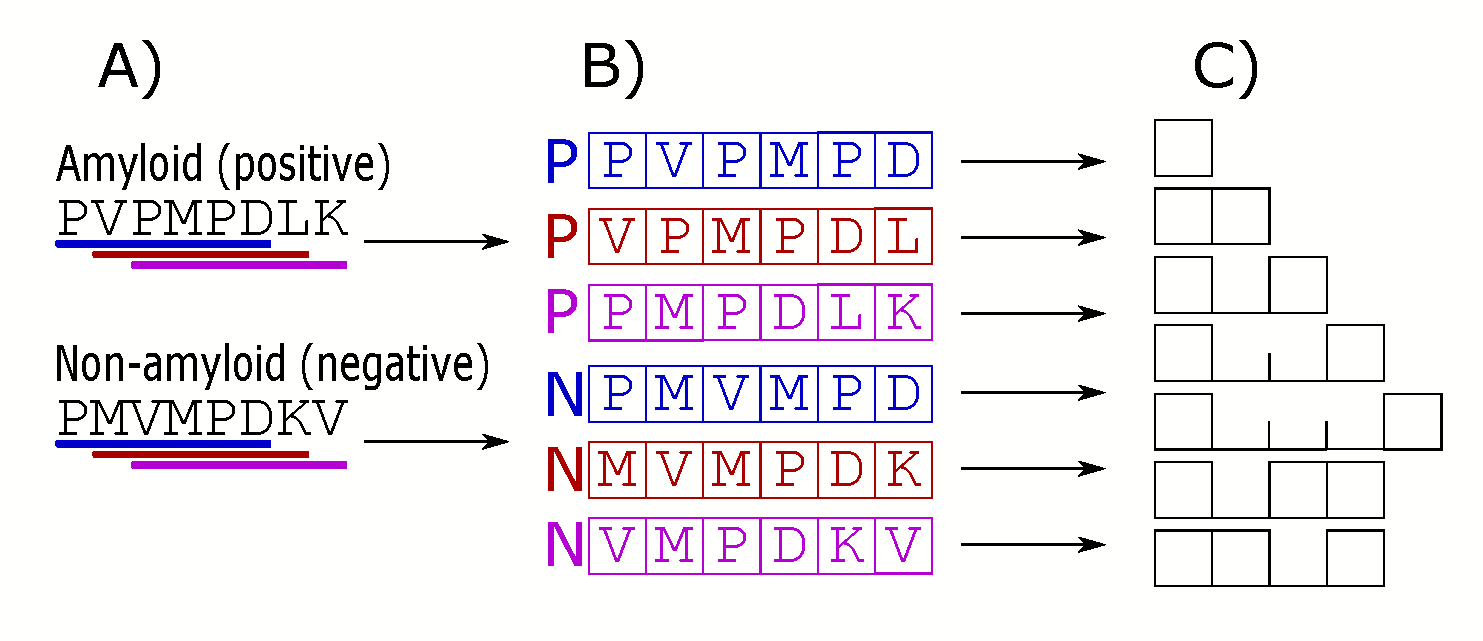
\includegraphics[width=\maxwidth]{ngram_scheme}
\end{figure}

\begin{enumerate}[1.]
\item Sequences shorter than 6 amino acids were discarded.
\item From each sequence overlapping windows of length 6 were extracted. All windows were labelled as their sequence of the origin, e.g. all windows extracted from amyloid sequence were labelled as positive (see Figure A and B).
\item For each window, 1-, 2- and 3-grams (both discontinous and continous) were extracted (see Figure B). For each encoding, the encoded n-grams were filtered by the QuiPT and used to train the Random Forests~\citep{liaw_classification_2002}. This procedure was performed independently on three training sets: a) 6 amino acids, b) 10 amino acids or shorter, c) 15 amino acids or shorter creating three classifiers.
\item All classifiers were evaluated in the 5-fold cross-validation eight times. The sequence was labelled as positive (amylogenic), if at least one window was assessed as amylogenic.
\end{enumerate}

\end{block}
\vfill

\begin{block}{Encoding distance}

The encoding distance between \textbf{A} and \textbf{B} is defined as the minimum number of amino acids that have to be shifted between subgroups of encoding \textbf{A} to make it identical to \textbf{B} (order of subgroups in the encoding and amino acids in a group is unimportant).

\begin{columns}
\column{.4\textwidth}
% latex table generated in R 3.2.2 by xtable 1.7-4 package
% Wed Sep 23 13:46:41 2015
\begin{table}[ht]
\centering
\begin{tabular}{c|l}
  \toprule
Group & Elements \\ 
  \midrule
1 & a, b, c \\ 
   \rowcolor[gray]{0.75}2 & d, e \\ 
   \bottomrule
\end{tabular}
\caption{Encoding \textbf{A}.} 
\end{table}

\column{.4\textwidth}

% latex table generated in R 3.2.2 by xtable 1.7-4 package
% Wed Sep 23 13:46:41 2015
\begin{table}[ht]
\centering
\begin{tabular}{c|l}
  \toprule
Group & Elements \\ 
  \midrule
1 & a, b \\ 
   \rowcolor[gray]{0.75}2 & d, e \\ 
  3 & c \\ 
   \bottomrule
\end{tabular}
\caption{Encoding \textbf{B}.} 
\end{table}

\end{columns}

The encoding distance between \textbf{A} and \textbf{B} is 1 (element \textit{c} must be moved from Group 3 to Group 1).

\end{block}
\vfill



}
\end{minipage}
\end{beamercolorbox}
\end{column}


%new column ------------------------------------------------------    

\begin{column}{.50\textwidth}
\begin{beamercolorbox}[center,wd=\textwidth]{postercolumn}
\begin{minipage}[T]{.95\textwidth}  
\parbox[t][\columnheight]{\textwidth}
{




\begin{block}{Specificity versus sensitivity}
% latex table generated in R 3.2.2 by xtable 1.7-4 package
% Wed Sep 23 13:46:41 2015
\begin{table}[ht]
\centering
\begin{tabular}{c|c|c|c|c|c}
  \toprule
Training length & Number of groups & Encoding ID & AUC & Specificity & Sensitivity \\ 
  \midrule
6 & 3 & 6 & 0.7955 & 0.8221 & 0.6181 \\ 
   \rowcolor[gray]{0.75}6 & 4 & 45 & 0.8183 & 0.9014 & 0.5038 \\ 
  $<$11 & 4 & 2 & 0.6615 & 0.4304 & 0.8307 \\ 
   \rowcolor[gray]{0.75}$<$11 & 3 & 15 & 0.8088 & 0.8329 & 0.6060 \\ 
  $<$16 & 3 & 16 & 0.8162 & 0.7477 & 0.7374 \\ 
   \rowcolor[gray]{0.75}$<$16 & 6 & 87 & 0.8320 & 0.5186 & 0.9195 \\ 
   \bottomrule
\end{tabular}
\caption{Encodings with the best sensitivity and specificity for each training set type.} 
\end{table}


The best specificity encoding (training length 6, 4 groups, encoding ID 45) and the best sensitivity (training length $<$16, 6 groups, encoding ID 87) seem to have the different areas of the competence.

The committee of the best specificity and best sensitivity classifiers has overall $0.8911$ AUC, $0.7473$ sensitivity and $0.8684$ specificity.

\end{block}
\vfill

\begin{block}{Bibliography}
  \tiny{
  \bibliographystyle{apalike}
  \bibliography{amyloids}
  }
  \end{block}
  \vfill

}
\end{minipage}
\end{beamercolorbox}
\end{column}
\end{columns}  
\end{frame}
\end{document}
